\appendix
\addtocontents{toc}{\protect\setcounter{tocdepth}{2}} %\TODO set appendix counter
\section{Appendix}

\subsection{Mathematical Tools and Defintions}

\subsubsection{Sherman-Morrison Formula}
\label{CH:Appendix:Math:MatrixInversion}

The Sherman-Morrison formula is based on the Woodbury Formula:

\begin{lemma}[Woodbury Formula]
    Let $E$ and $G$ be square invertible matrices of dimension $n_E \times n_E$ and $n_G \times n_G$ respectively. Let $F$ and $H$ be matrices of size $n_E \times n_G$ and $n_G \times n_E$ respectively, then the following identity holds:
    \begin{equation}
        (E + FGH)^{-1} = E^{-1} - E^{-1} F(G^{-1} + HE^{-1}F)^{-1}HE^{-1} \label{EQ:Woodbury}
    \end{equation}
\end{lemma}

The Sherman-Morrison formula is a special case of \refp{EQ:Woodbury} where $G = 1$ and $F=u \in \R^{n_E}$ and $H=v \in \R^{n_E}$ which results in the equality
\begin{equation}
    (E+uv')^{-1} = E^{-1} - \frac{E^{-1}uv'E^{-1}}{1 + v'E^{-1}u}
\end{equation}
For the case of the recursive least squares this translates equation \refp{EQ:RLS11} into \refp{EQ:RLS21}.

\subsubsection{Standard Brownian Motion}

A stochastic process $\left(B_t\right)_{t\geq0}$ that satisfies
\begin{enumerate}
    \item $B_0 = 0 \,\,\mathbb{P}\textit{-almost surely, e.g. } \mathbb{P}\left(\omega \in \Omega : B\left(0,\omega\right) \neq 0 \right) = 0 $.
    \item $\textit{The increments } B_t - B_s \textit{ for } t>s \textit{ follow a normal distribution } \mathcal{N}(0,t-s)$.
    \item $\textit{For all } 0\leq t_1 < t_2 < ... < t_n \textit{ it holds that } B_{t_2} - B_{t_1}, \, ... \, ,B_{t_n}-B_{t_{n-1}} \\ \textit{are independent}$.
\end{enumerate}
is called Brownian Motion or Wiener Process.

\subsection{Single ESN predictive performance}

These are the predictive performances of a single ESN of equivalent size to the experts approach, namely $N=1000$ internal neurons. The hyperparameters that have been tuned are the spectral radius and the bias in the interval $\rho \in (0, 3]$ and bias $b \in [-1,1]$ using a gradient boosted regression tree from the scikit-optimize package. See the appendix for details.

\begin{figure}[H]
    \begin{center}
        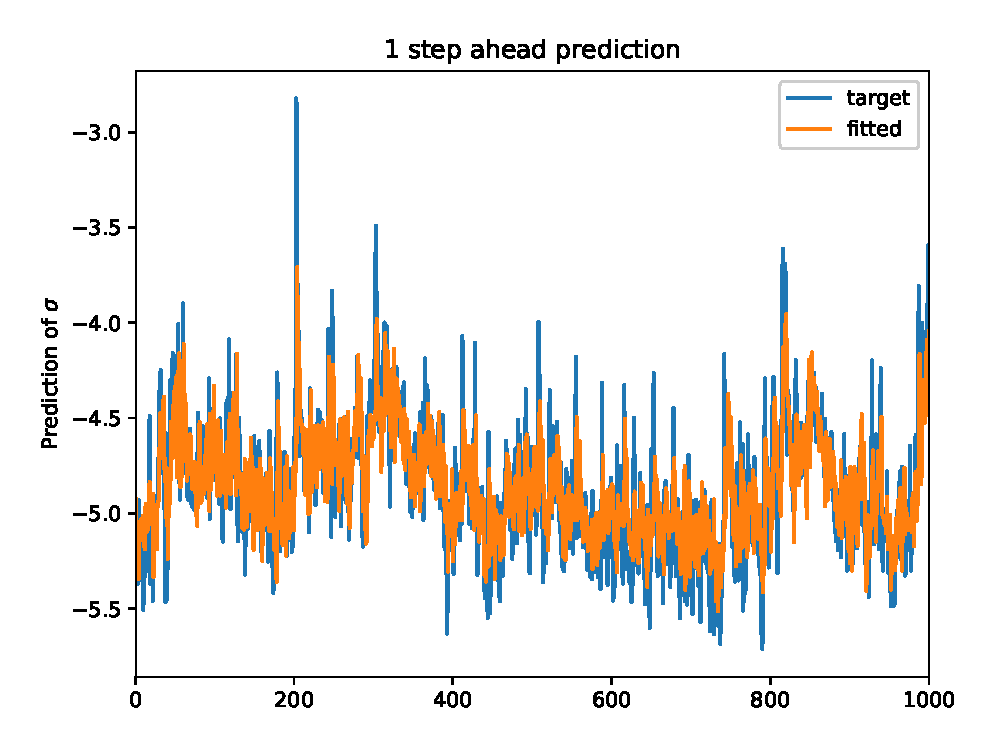
\includegraphics[width=0.45\textwidth]{Plots/Prediction/Single_logMSE_1step.eps}
        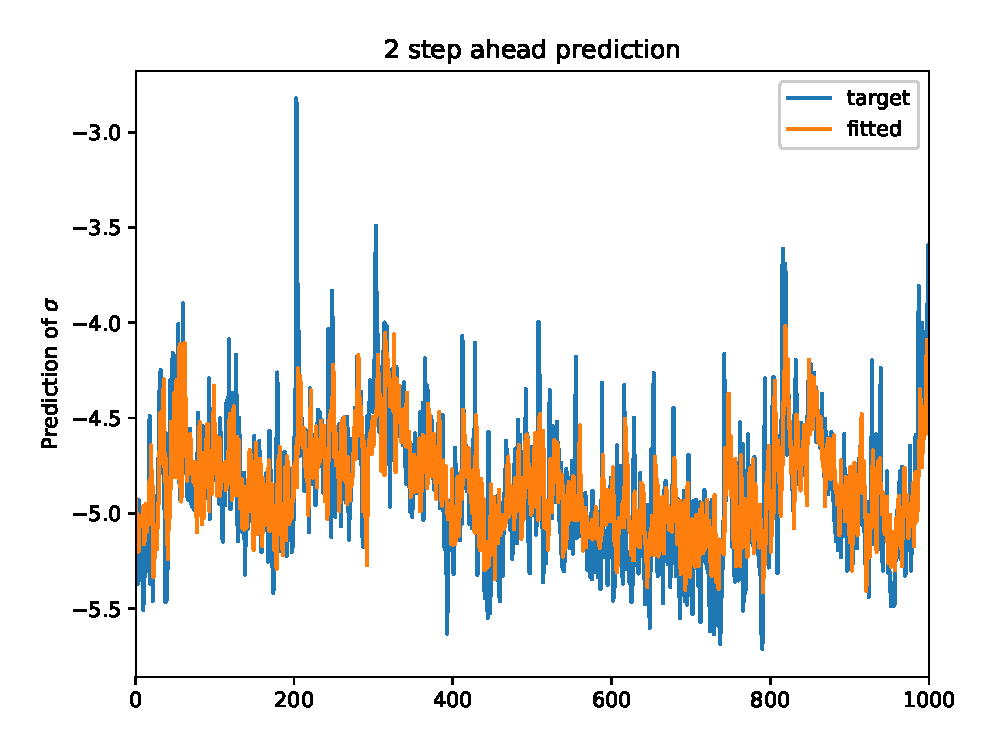
\includegraphics[width=0.45\textwidth]{Plots/Prediction/Single_logMSE_2step.eps} \\
        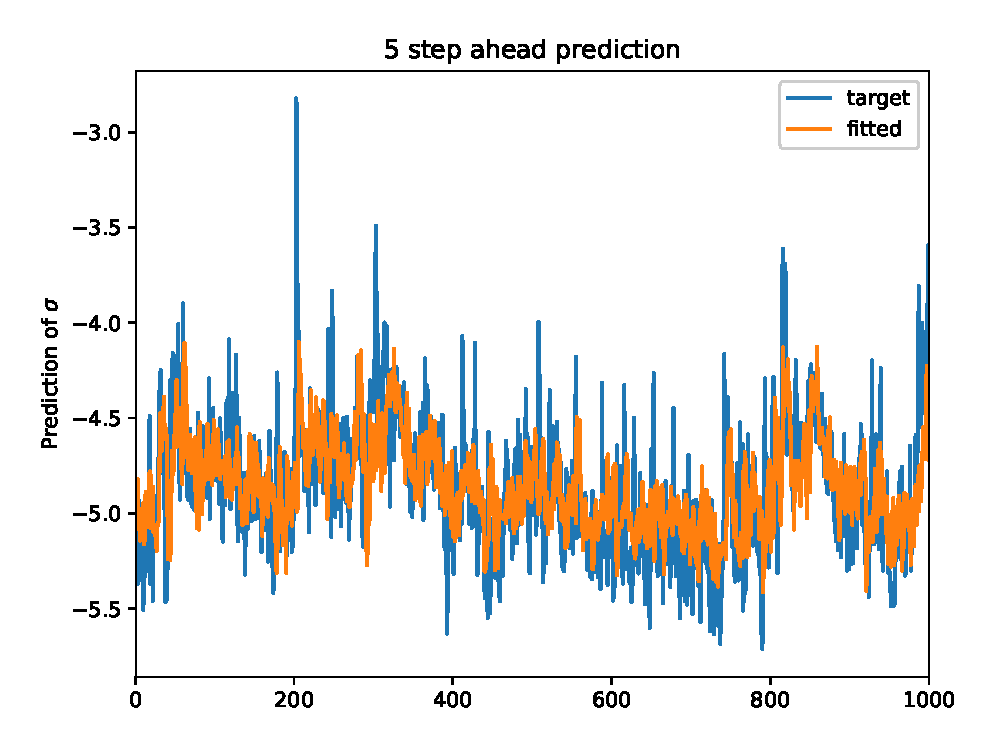
\includegraphics[width=0.45\textwidth]{Plots/Prediction/Single_logMSE_5step.eps}
        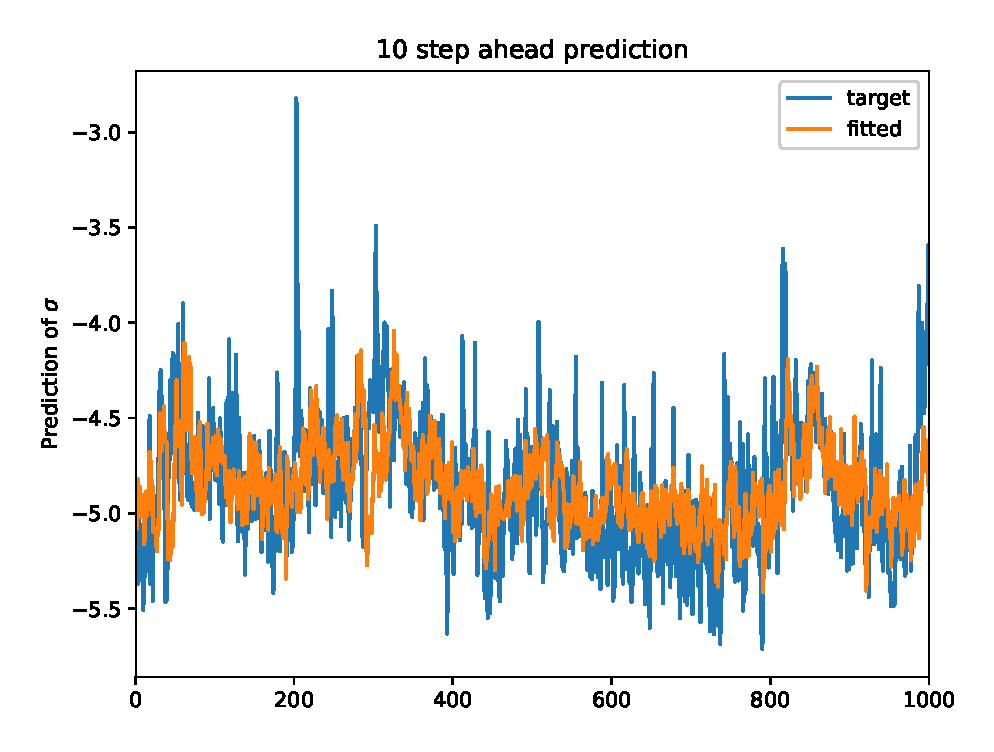
\includegraphics[width=0.45\textwidth]{Plots/Prediction/Single_logMSE_10step.eps}
    \end{center}
    \caption{Single Echo State Network using the logMSE as error function in the cross-validation.}
    \label{FIG:SingleESNlogMSE}
\end{figure}

\begin{figure}[H]
    \begin{center}
        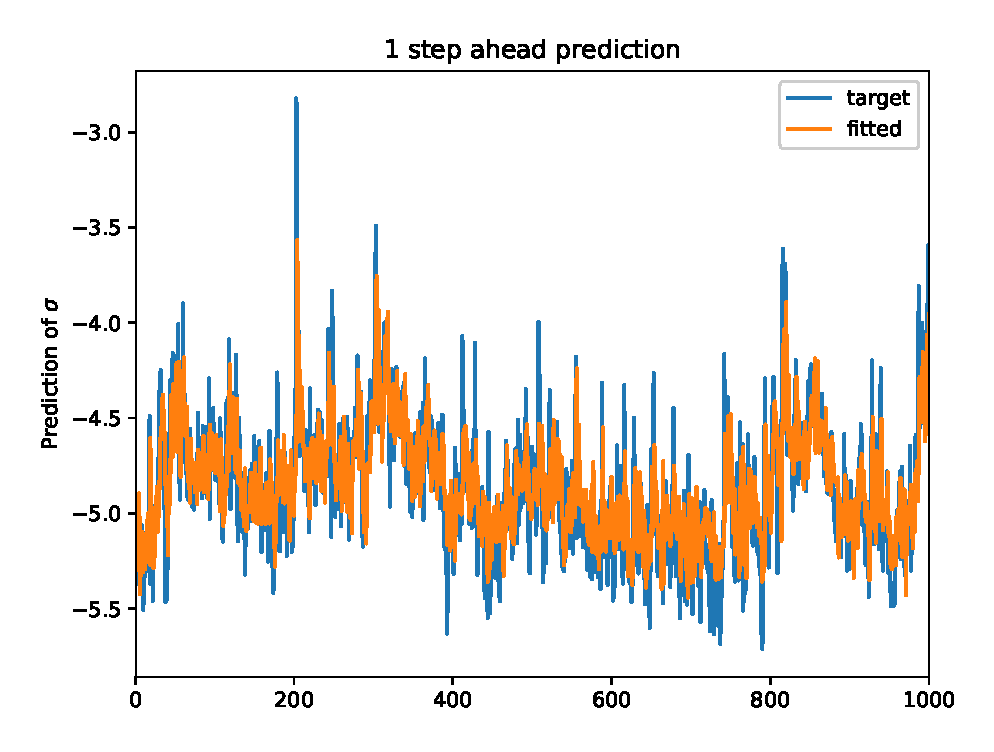
\includegraphics[width=0.45\textwidth]{Plots/Prediction/Single_QLIKE_1step.eps}
        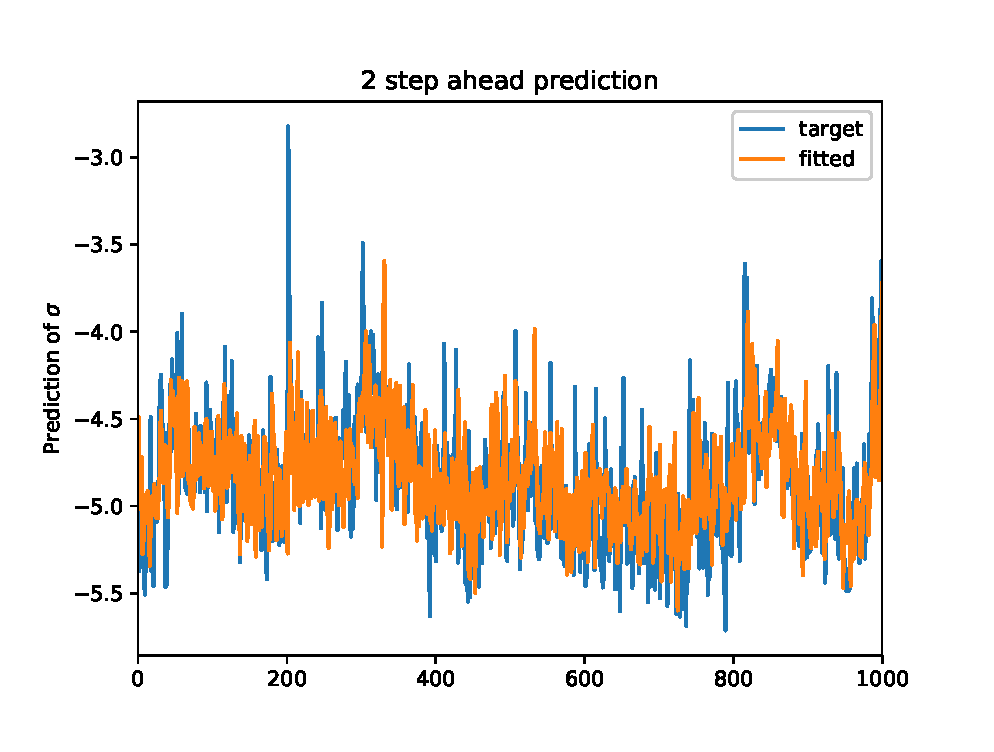
\includegraphics[width=0.45\textwidth]{Plots/Prediction/Single_QLIKE_2step.eps} \\
        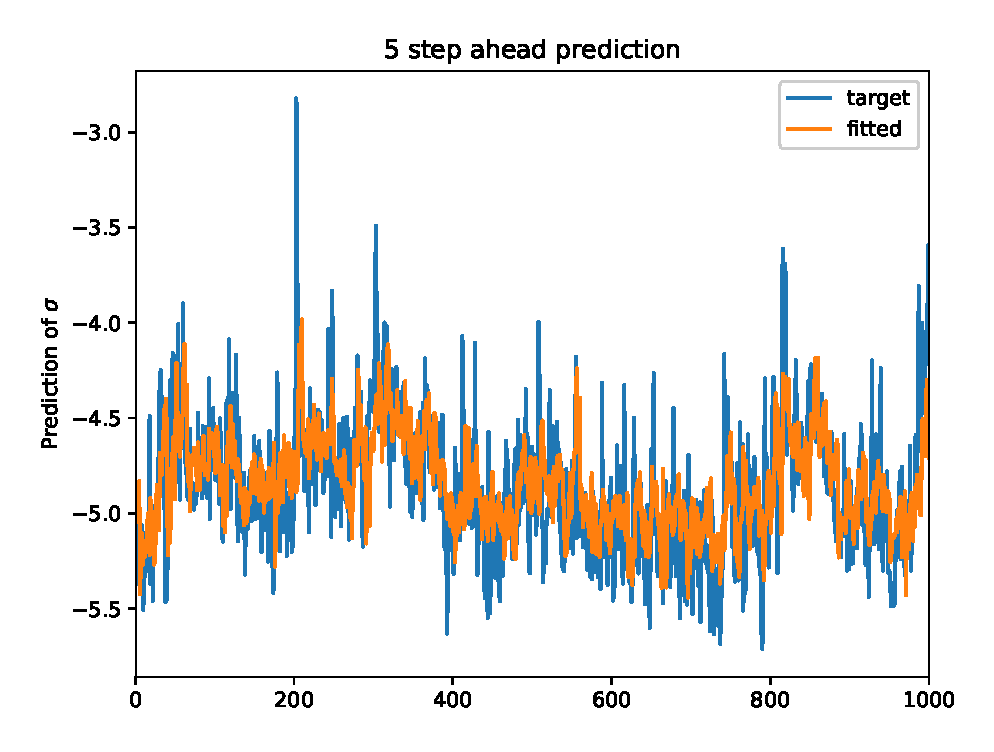
\includegraphics[width=0.45\textwidth]{Plots/Prediction/Single_QLIKE_5step.eps}
        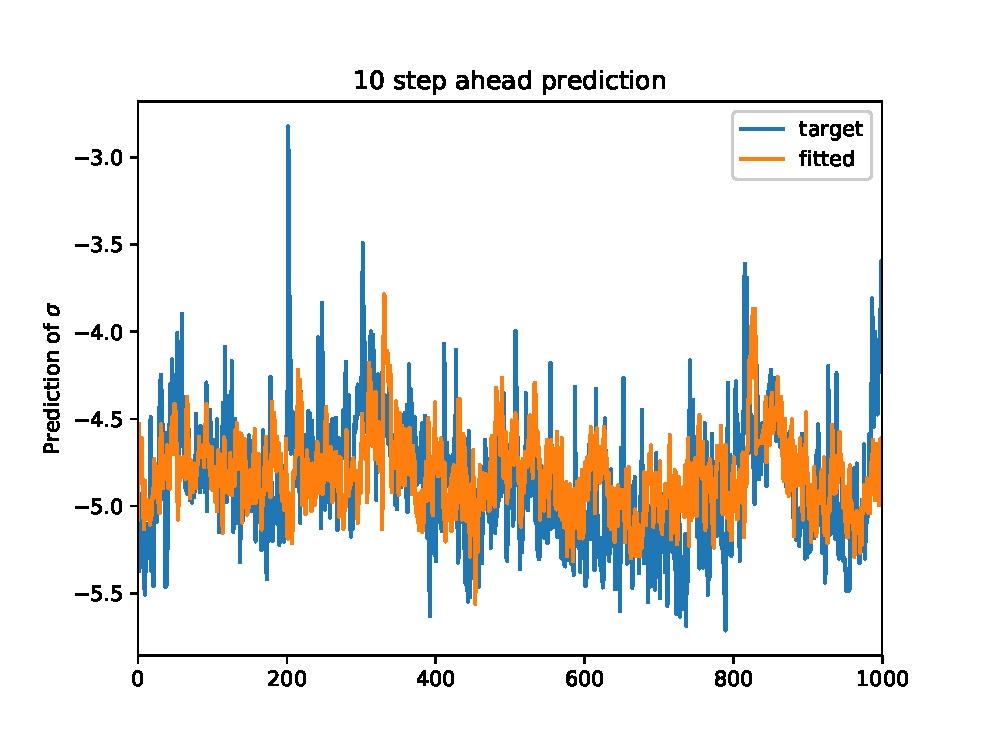
\includegraphics[width=0.45\textwidth]{Plots/Prediction/Single_QLIKE_10step.eps}
    \end{center}
    \caption{Single Echo State Network using the QLIKE as error function in the cross-validation.}
    \label{FIG:SingleESNQLIKE}
\end{figure}


\subsection{Grid of Smaller Sigma Values}
\label{CH:Appendix:GridSmallerSigma}



\begin{figure}[H]
    \begin{center}
        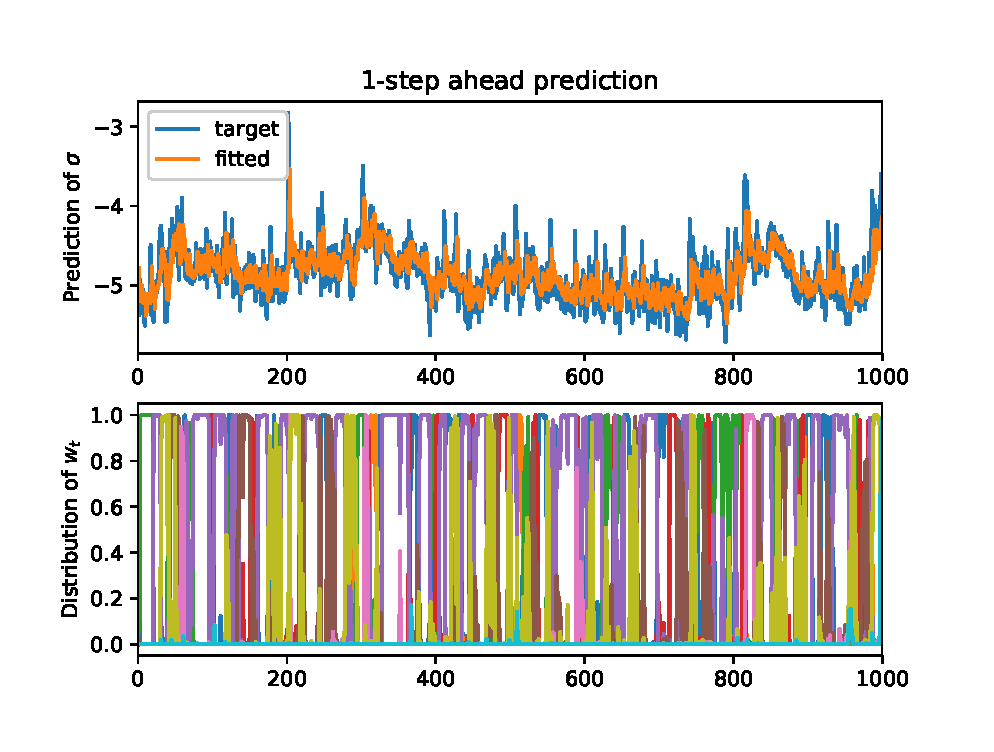
\includegraphics[width=0.45\textwidth]{Plots/Prediction/Plasticity_Constant_Middle_rolling_1step.eps}
        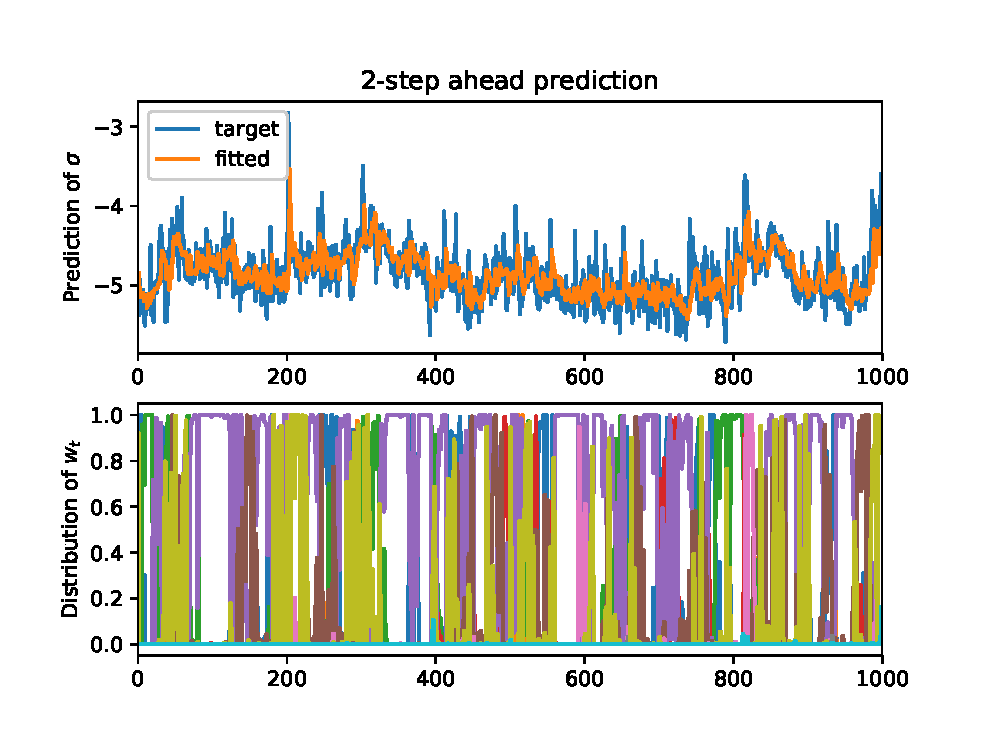
\includegraphics[width=0.45\textwidth]{Plots/Prediction/Plasticity_Constant_Middle_rolling_2step.eps} \\
        \includegraphics[width=0.45\textwidth]{Plots/Prediction/Plasticity_Constant_Middle_rolling_5step.eps}
        \includegraphics[width=0.45\textwidth]{Plots/Prediction/Plasticity_Constant_Middle_rolling_10step.eps} \\
        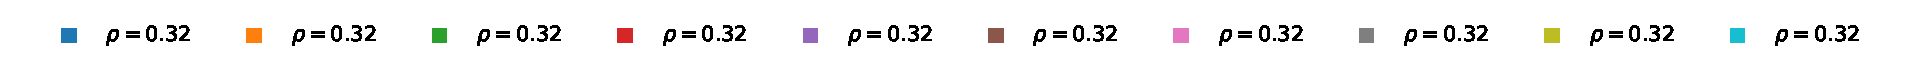
\includegraphics[width=1.0\textwidth]{Plots/Prediction/legend_Constant_Middle.eps}
    \end{center}
    \caption{This presents the predictive performance of the \textit{plasticity experts} for 1, 2, 5 and 10 step ahead predictions. The targeted network activations are using a constant $\sigma = 0.32$ for all networks based on the dominate weight of this network in the grid approach of section \ref{CH:EmpiricalResults:Rolling}.}
    \label{FIG:PlasticityConstantMiddle}
\end{figure}

\begin{figure}[H]
    \begin{center}
        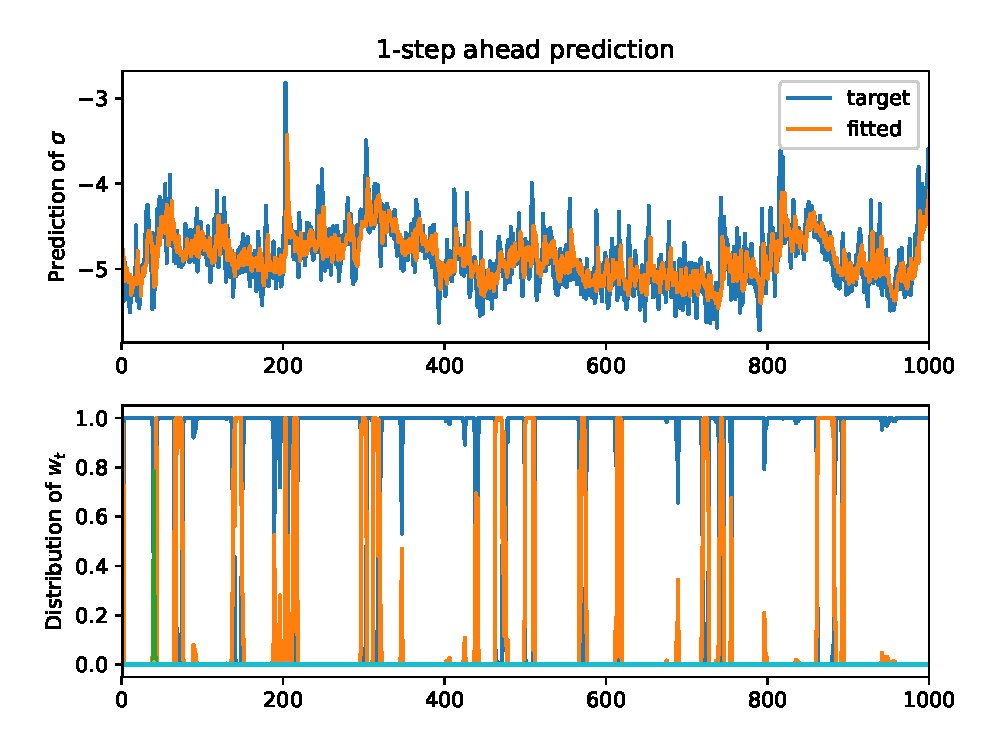
\includegraphics[width=0.45\textwidth]{Plots/Prediction/Plasticity_Grid_Middle_rolling_1step.eps}
        \includegraphics[width=0.45\textwidth]{Plots/Prediction/Plasticity_Grid_Middle_rolling_2step.eps} \\
        \includegraphics[width=0.45\textwidth]{Plots/Prediction/Plasticity_Grid_Middle_rolling_5step.eps}
        \includegraphics[width=0.45\textwidth]{Plots/Prediction/Plasticity_Grid_Middle_rolling_10step.eps} \\
        \includegraphics[width=1.0\textwidth]{Plots/Prediction/legend_Grid_Middle.eps}
    \end{center}
    \caption{This presents the predictive performance of the \textit{plasticity experts} for 1, 2, 5 and 10 step ahead predictions. The targeted network activations are using an equally spaced grid $\left[0.26, 0.35\right]$ around the constant $\sigma = 0.32$ based on the dominate weight of this network in the grid approach of section \ref{CH:EmpiricalResults:Rolling}.}
    \label{FIG:PlasticityGridMiddle}
\end{figure}

\begin{figure}[H]
    \begin{center}
        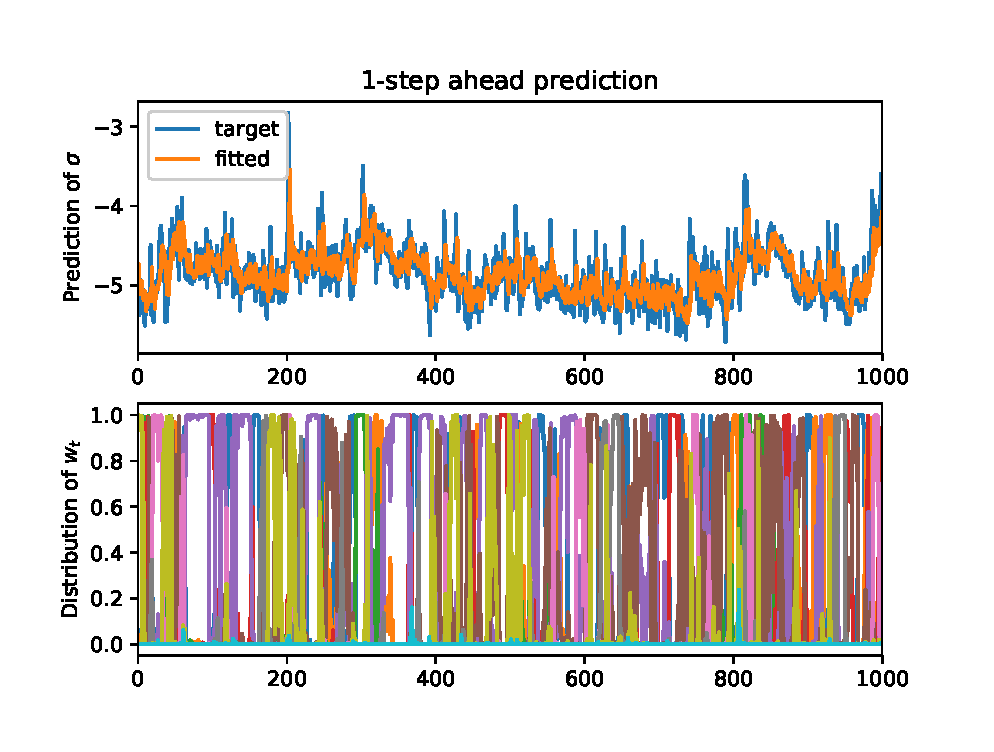
\includegraphics[width=0.45\textwidth]{Plots/Prediction/Plasticity_Constant_Low_rolling_1step.eps}
        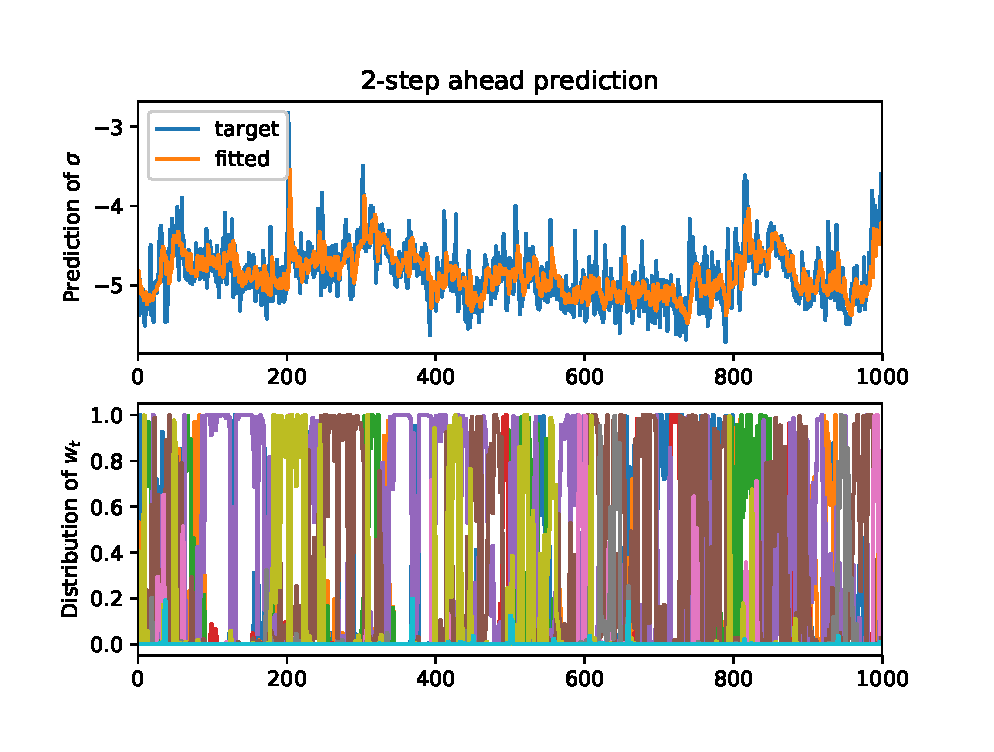
\includegraphics[width=0.45\textwidth]{Plots/Prediction/Plasticity_Constant_Low_rolling_2step.eps} \\
        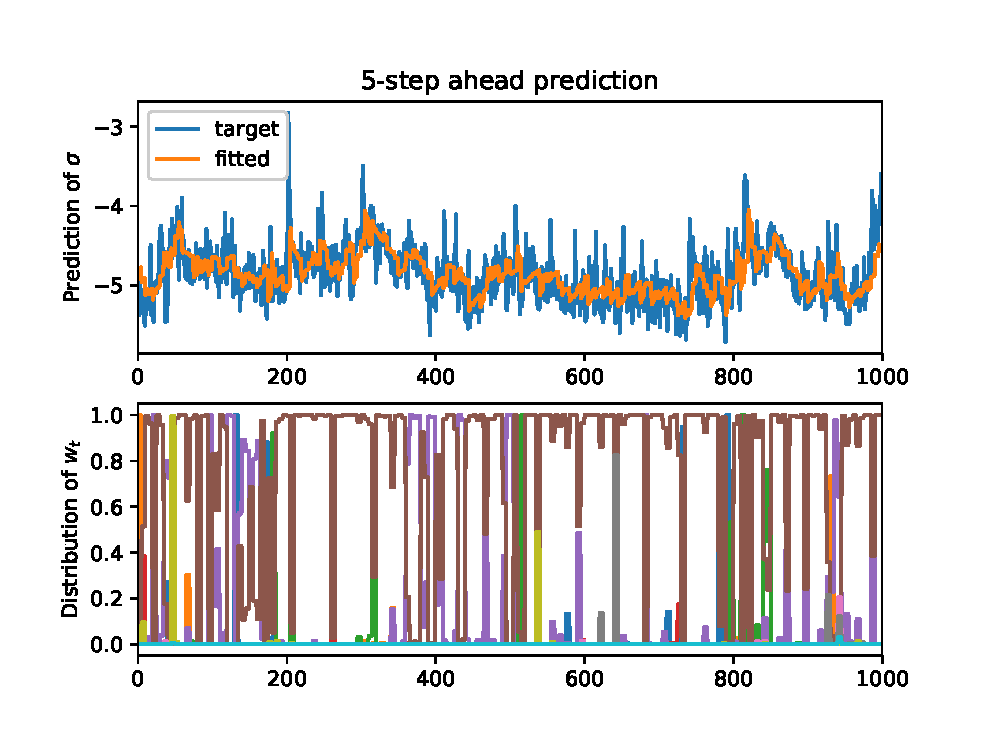
\includegraphics[width=0.45\textwidth]{Plots/Prediction/Plasticity_Constant_Low_rolling_5step.eps}
        \includegraphics[width=0.45\textwidth]{Plots/Prediction/Plasticity_Constant_Low_rolling_10step.eps} \\
        \includegraphics[width=1.0\textwidth]{Plots/Prediction/legend_Constant_Low.eps}
    \end{center}
    \caption{This presents the predictive performance of the \textit{plasticity experts} for 1, 2, 5 and 10 step ahead predictions. The targeted network activations are using a constant $\sigma = 0.21$ for all networks based variance of the underlying series of realized volatility.}
    \label{FIG:PlasticityConstantLow}
\end{figure}

\begin{figure}[H]
    \begin{center}
        \includegraphics[width=0.45\textwidth]{Plots/Prediction/Plasticity_Grid_Low_rolling_1step.eps}
        \includegraphics[width=0.45\textwidth]{Plots/Prediction/Plasticity_Grid_Low_rolling_2step.eps} \\
        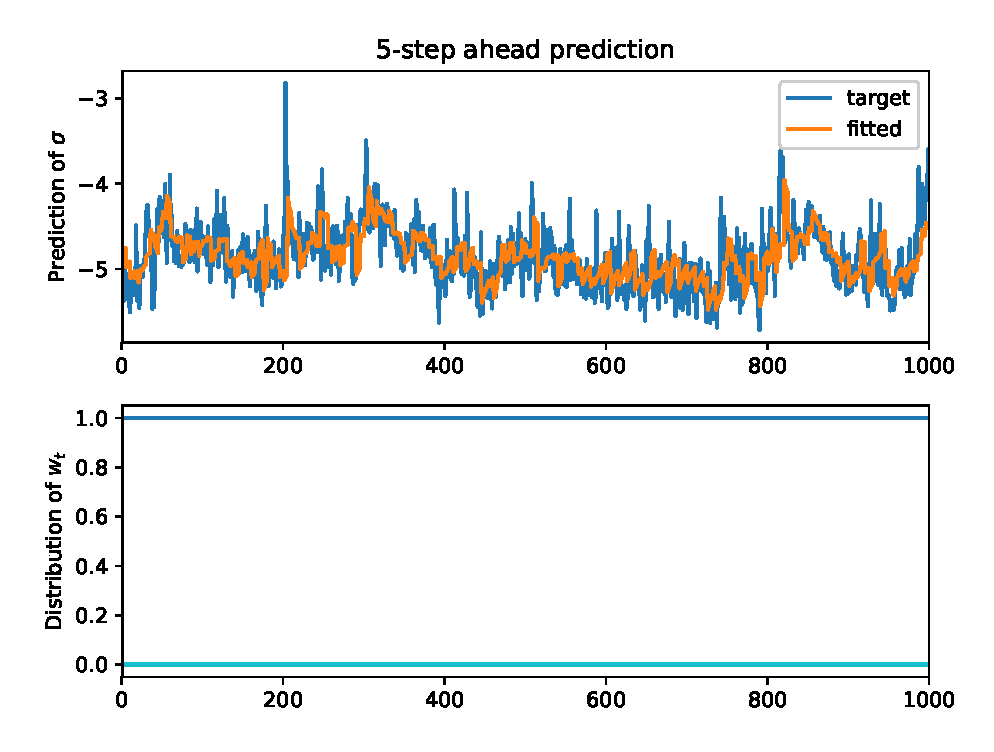
\includegraphics[width=0.45\textwidth]{Plots/Prediction/Plasticity_Grid_Low_rolling_5step.eps}
        \includegraphics[width=0.45\textwidth]{Plots/Prediction/Plasticity_Grid_Low_rolling_10step.eps} \\
        \includegraphics[width=1.0\textwidth]{Plots/Prediction/legend_Grid_Low.eps}
    \end{center}
    \caption{This presents the predictive performance of the \textit{plasticity experts} for 1, 2, 5 and 10 step ahead predictions. The targeted network activations are using an equally spaced grid $\left[0.15, 0.24\right]$ around the constant $\sigma =0.21$ based variance of the underlying series of realized volatility.}
    \label{FIG:PlasticityGridLow}
\end{figure}

Choosing the new alternative constant value of $\sigma$ or the shifted grid, doesn't change the weight distribution of and their behaviour. For the constant value of $\sigma$ the distributions are still very volatile. For the shifted grid of values for $\sigma$ it turns out, that still the weights are distributed between the lowest $\sigma$ network and the second lowest $\sigma$. This leads to the conclusion that likelihood of the network state is in fact reliant on the random weights of the internal connections and the plasticity tuning of the networks connections are not 

Choosing the new constant value of $\sigma = 0.32$ doesn't improve the network performance significantly. Shifting the grid doesn't change much in the weight distribution.

In the grid approach with a lower grid of values, still the network with the lowest $\sigma$ receives the largest weight.


\begin{table}[H]
    \begin{center}
        \begin{tabular}{r|c|c|c}
            & Original & Middle & Low \\\hline
            Constant & $\frac{1}{\sqrt{2\pi}} \approx 0.40$ & 0.32 & 0.21 \\\hline
            Grid & $\left[0.8\frac{1}{\sqrt{2\pi}}, 1.2\frac{1}{\sqrt{2\pi}}\right]$ & $\left[0.26, 0.35\right]$ & $\left[0.15, 0.24\right]$ 
        \end{tabular}
    \end{center}
    \caption{Reference for the following tables}
\end{table}

\begin{table}[H]
    \begin{center}
        
\begin{tabular}{l|c|c|c}
Rolling 1-step ahead     & logMSE & MSE $(\times 10^{-5})$ & QLIKE \\\hline
Plasticity Constant Middle & 0.08726152 & 1.02852912 & 0.25950733\\ 
Plasticity Constant Low & 0.08637962 & 1.01789215 & 0.25328345\\ 
Plasticity Constant & 0.08742805 & 1.03377312 & 0.25916568\\ 
Plasticity Grid Low & 0.08942995 & 1.03451887 & 0.25295346\\ 
Plasticity Grid Middle & 0.08599342 & 1.02120263 & 0.25862333\\ 
Plasticity Grid & 0.08620444 & 1.02328620 & 0.25938944\\ 
\end{tabular}
    \end{center}
    \caption{Errors for the rolling prediction for the different models and the $1$-step ahead predictions.}
    \label{TABLE:Appendix:1step}
\end{table} 

\begin{table}[H]
    \begin{center}
        
\begin{tabular}{l|c|c|c}
Rolling 2-step ahead     & logMSE & MSE $(\times 10^{-5})$ & QLIKE \\\hline
Plasticity Constant Low & 0.08736678 & 1.03018180 & 0.25832888\\ 
Plasticity Constant Middle & 0.08816717 & 1.04446062 & 0.26580909\\ 
Plasticity Constant & 0.08822185 & 1.04517222 & 0.26429428\\ 
Plasticity Grid Low & 0.09136562 & 1.06222826 & 0.26008277\\ 
Plasticity Grid Middle & 0.08762366 & 1.04400969 & 0.26553307\\ 
Plasticity Grid & 0.08736104 & 1.04320714 & 0.26452248\\ 
\end{tabular}
    \end{center}
    \caption{Errors for the rolling  prediction for the different models and the $2$-step ahead predictions.}
    \label{TABLE:Appendix:2step}
\end{table} 

\begin{table}[H]
    \begin{center}
        
\begin{tabular}{l|c|c|c}
Rolling 5-step ahead     & logMSE & MSE $(\times 10^{-5})$ & QLIKE \\\hline
Plasticity Constant Low & 0.09721939 & 1.13024216 & 0.31649472\\ 
Plasticity Constant Middle & 0.09780792 & 1.13913434 & 0.31888618\\ 
Plasticity Constant & 0.09802419 & 1.14526361 & 0.31551162\\ 
Plasticity Grid Low & 0.10543143 & 1.18778672 & 0.34084742\\ 
Plasticity Grid Middle & 0.09543957 & 1.11023250 & 0.30987966\\ 
Plasticity Grid & 0.09590954 & 1.11738107 & 0.30815891\\ 
\end{tabular}
    \end{center}
    \caption{Errors for the rolling  prediction for the different models and the $5$-step ahead predictions.}
    \label{TABLE:Appendix:5step}
\end{table} 

\begin{table}[H]
    \begin{center}
        
\begin{tabular}{l|c|c|c}
Rolling 10-step ahead     & logMSE & MSE $(\times 10^{-5})$ & QLIKE \\\hline
Plasticity Constant Low & 0.10915696 & 1.22575270 & 0.35292040\\ 
Plasticity Constant Middle & 0.11126106 & 1.25985877 & 0.36134648\\ 
Plasticity Constant & 0.11459149 & 1.30729493 & 0.36355034\\ 
Plasticity Grid Low & 0.12052321 & 1.30609972 & 0.37401721\\ 
Plasticity Grid Middle & 0.10630105 & 1.19898912 & 0.33948644\\ 
Plasticity Grid & 0.10688234 & 1.20814290 & 0.34068571\\ 
\end{tabular}
    \end{center}
    \caption{Errors for the rolling  prediction for the different models and the $10$-step ahead predictions.}
    \label{TABLE:Appendix:10step}
\end{table} 

Changing the exact distribution of the targeted output distributions doesn't affect the performance very much. The best improvement could be achieved in teh 'Plasticity Constant Low' for all different prediction steps when comparing to the original 'Plasticity Constant'. In terms of the grids of output distributions, the 'Plasticity Grid Middle' seems to improve the performance slightly. Alltogether there is a tendency that lower variance for the targeted output distributions may be preferrable to the one chosen in the empirical appplication. One possible explanation may be based on the variance which is around $0.21$ for the whole dataset (training and testing). Another explanation may be, that the network is generally more capable of achieving output distributions with lower targeted variances. After all, given that the improvements are minor, a more rigurous analysis has to be conducted to support any specific choices of the output distributions.


\subsection{Implementation}
All implementations have been self written in Python where the main engine behind the code is \textit{NumPy} (\url{https://numpy.org}) and no other high level libraries like \textit{Tensorflow/Keras} (\url{https://tensorflow.org}) or \textit{pyTorch} (\url{https://pytorch.org}) have been used.
Link to the GitHub repository:
\begin{center}
    lucasburger.github.io/pyRC
\end{center}


\subsubsection{Python's Scikit-Optimize}
\label{A:ScikitOptimize}

This section of the appendix is for some more light and details on how the python package was employed for the optimization of hyperparameters. In addition, we refer to the online presentation of the package under \url{https://scikit-optimize.github.io/stable/}. The following is mainly stated from this website:
The package provides different optimizers which include the following models to approximate the expensive to evaluate function:
\begin{multicols}{2}
\begin{itemize}
\item {\bf dummy{\_}minimize}:\\ This is basic grid search
\item {\bf gp{\_}minimize}:\\ Gaussian Process
\item {\bf gbrt{\_}minimize}:\\ Gradient Boosted Regression Trees
\item {\bf forest{\_}minimize}:\\ Tree Based regression
\end{itemize}
\end{multicols}
One can set multiple parameters in order to run the optimization. Required arguments are the function that one want to minimize and the dimensions and ranges to use. There are many other parameters to direct the optimization onto different paths, but all of them do have default values and don't necessarily need any attention.
Visualization of the results is very easy as well and includes, among others, the diagnostics presented in figure \ref{FIG:ScikitExample}. For this example, the spectral radius and the leak of an ESN applied on the Mackey-Glass time series have been optimized. Convergence has been pretty fast, because it only took aroung $40$ function evalutations.
\begin{figure}[H]
\begin{center}
\includegraphics[width=0.48\textwidth]{Plots/ScikitOptimizeConvergence.eps}
\includegraphics[width=0.48\textwidth]{Plots/ScikitOptimizeObjective.eps}
\end{center}
\caption{On the left, we have the convergence plot of the function evaluations. On the right, we can see the partial dependence of two variables in rlation to each other. Blue dots represent functionevaluations and the red dot (barely recognizable in the top left corner) is the final value pair.}
\label{FIG:ScikitExample}
\end{figure}




\subsection{Mackey Glass Time Series and Network Dynamics}

The Mackey-Glass differential equation \citep{MackeyGlass2010Scholar}
\begin{equation}
x'(t) = b \frac{x(t-\tau)}{1+x(t-\tau)^n}-c x(t) \quad , \quad t \in \R
\end{equation}
for $b, c, \tau, n \in \R$ can be adjusted to generate complex dynamics. 

\label{A:MackeyGlassESN}
Figure \ref{FIG:MackeyGlassExample} presents the Mackey-Glass time series for different values of the time-delay value $\tau$.
\begin{figure}[H]
\begin{center}
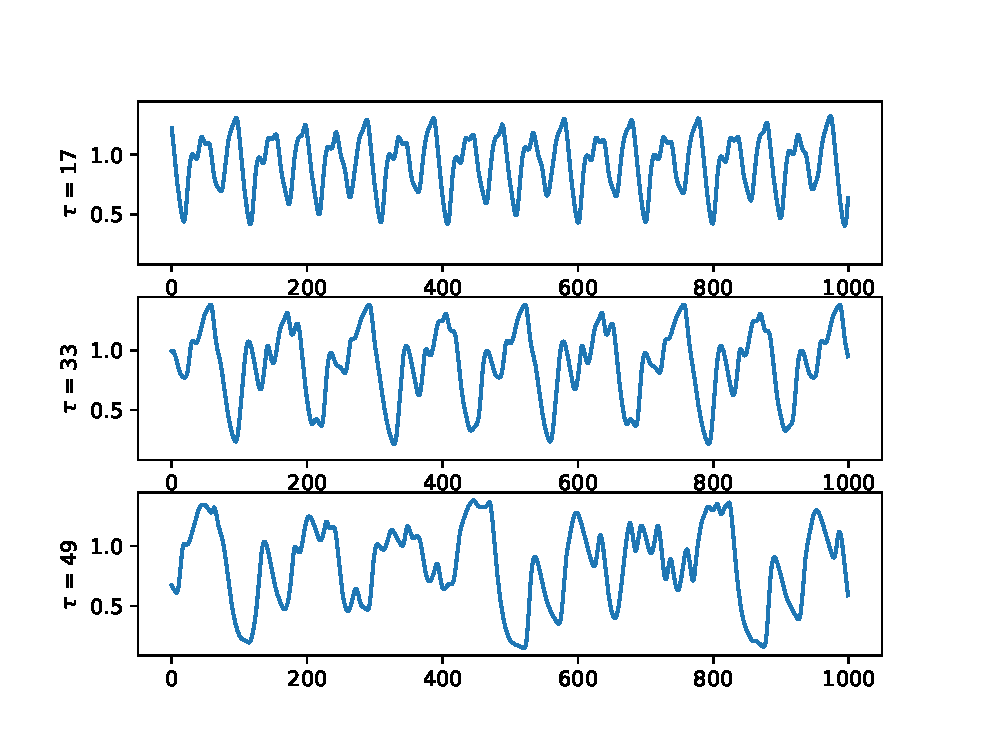
\includegraphics[width=0.8\textwidth]{Pictures/MackeyGlassExample.eps}
\end{center}
\caption{Examples of the Mackey-Glass time series. Depending on the time-delay value of $\tau$. Examples have been initialized with random values drawn from a uniform $\mathcal{U}(0.5, 1)$ that have been washed out over the simulation of $12000$ points. Plots show the last $1000$ of the simulations. Parameters are $b = 0.2$, $c = 0.1$, $n=10$ and $\tau \in \left\{17, 33, 49\right\}$ as indicated in the plot. One can clearly see the effect on irregularity when increasing $\tau$.}
\label{FIG:MackeyGlassExample}
\end{figure}

The neuron activations in figure \ref{A:NeuronActivation} indeed show certain similarities to the original time series which underlines the fact that the reservoir is able to reproduce different frequencies through its random, but well tuned weights. Depending on the input signal, the maginitude of neuron activations would be larger as well (there were also neurons with more variablity but they have been excluded from the plot).

\begin{figure}[H]
\begin{center}
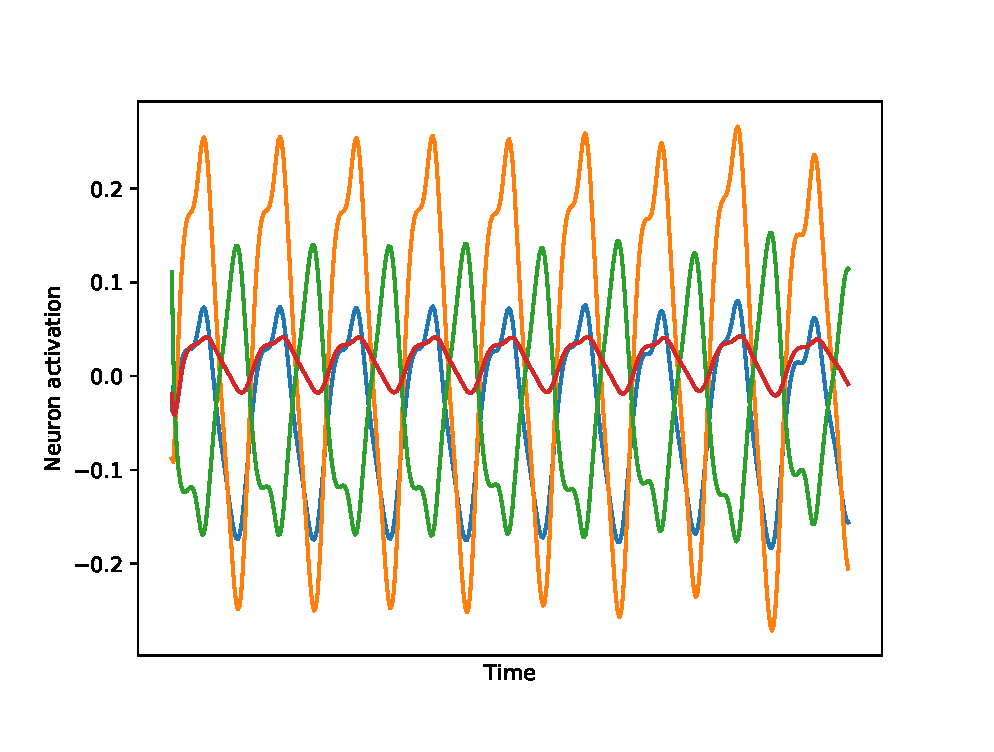
\includegraphics[width=0.8\textwidth]{Pictures/MackeyGlassNeuronExample.eps}
\end{center}
\caption{Exemplary neuron activation when feeding the Mackey-Glass time series with $\tau = 17$. This shows that the neurons are able to present different representations of the input signal. Neurons have been selected based on their range to be able to nicely present them. Some neurons with much larger variations did exist as well.} 
\label{A:NeuronActivation}
\end{figure}


\newpage